% Chapter Template

\chapter{Timeline for Degree Completion} % Main chapter title
%this should end up being roughly 2-3 pages
\label{Chapter5} % Change X to a consecutive number; for referencing this chapter elsewhere, use \ref{ChapterX}



\section{Gaant Chart}
The work described in my quantitative section, chapter \ref{sec:chapter3} and section \ref{sec:ch4_paper1} was submitted to \textit{Transactions in Geographic Information Science} on 15 March 2024, and is currently under review (shown in blue in figure \ref{monthly_gantt_chart}).  This is important in subsequent phases of my dissertation.  This initial research is responsible for generating a significant portion of the data required for follow on phases.  This included the selection, download, and pre-processing of over 4 TB of satellite imagery data. The amount of work invested in constructing this data set, should facilitate the ambitious timeline I present to support a May 2025 graduation (see figure \ref{monthly_gantt_chart}). 

Specifically, the first paper included preliminary work into explainability in satellite imagery.  The goal of the second phase of the research (purple in figure \ref{monthly_gantt_chart}) is to identify specific features in the image that might be important in classification of the image as either a riot or not.  The first two tasks in this are to gather point of interest data from Overture Maps \citep{OvertureMapsFoundation2023}, and to segment the pixels of interest from the Score-CAM analysis.  These two tasks can be accomplished concurrently during the month of April, given current progress.  During May, I will work on an algorithm which integrates points of interest with the pixels of interest to determine patterns of physical features on the ground that the trained ResNet has learned to associate with riots or null riots.  A goal of completing this phase by the summer of 2024, should be attainable and provide a much richer understanding of explainability as it pertains to satellite imagery.

The third chapter of my dissertation (orange in figure \ref{monthly_gantt_chart}) involves identifying conflict from contiguous satellite images, contrasted with classification of smaller 1\textit{$\ km^{2}$} boxes in the first phase.  The first task in this phase is to determine the appropriate methodology to segment full satellite images into a grid for subsequent conflict searches.  This effort should begin in July 2024.  By August, I will be training neural networks to detect riots within these full satellite scenes.  This will likely result in refinement in either the grid segmentation of satellite scenes, or the training of neural networks.  Depending on the initial results of this, there is a potential that I will have to increase the volume of my current data set or alter my methodology.  My current plan is to be complete with this research effort by the end of 2024.


I propose the following anticipated timeline, with consideration given to the dissertation milestones (indicated in green in Figure \ref{monthly_gantt_chart}), which are aligned to support a graduation in May 2025. In my initial paper, I aim to contribute to the body of literature on deep learning, conflict, and the classification of satellite imagery in urban environments. Subsequently, my second paper will delve into novel areas of explainability within the context of satellite imagery. Lastly, in my third paper, I plan to broaden the scope of my research by extending the functionality from analyzing small urban areas to encompassing comprehensive satellite scenes of larger areas.



\begin{figure}
    \centering
    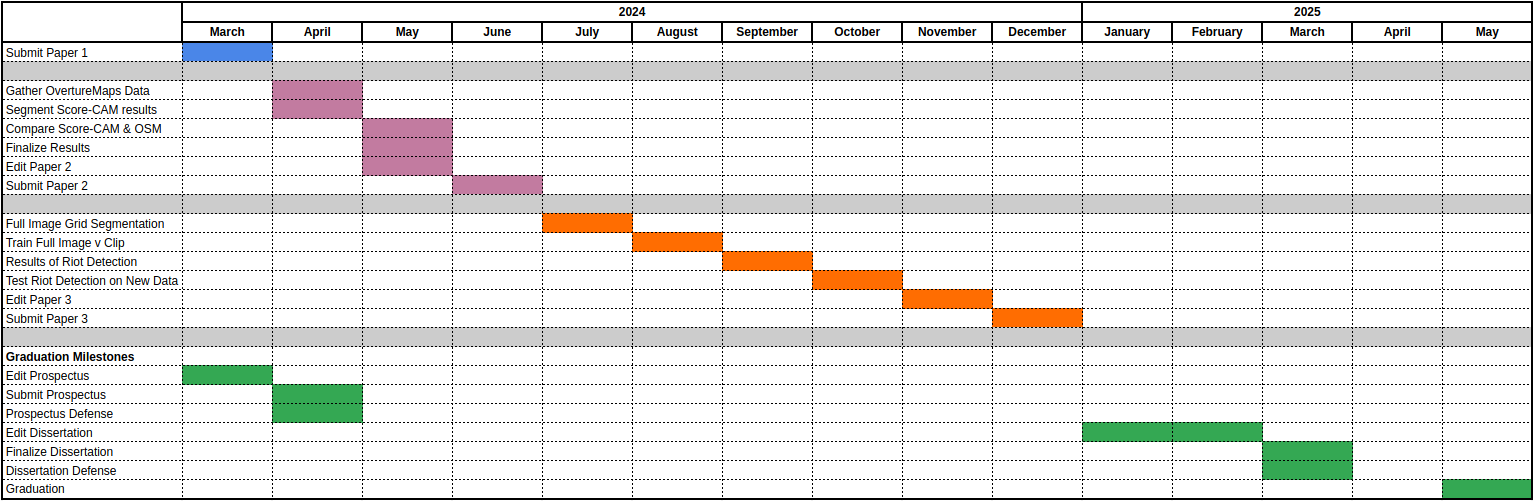
\includegraphics[width=1\linewidth]{Figures/monthly_gantt_chart.png}
    \caption{Gantt Chart supporting a May 2025 graduation. }
    \label{monthly_gantt_chart}
\end{figure}

